% =============================================================================
% SECCIÓN: CONEXIÓN CON LA TESIS
% =============================================================================
\section{Conexión con la Tesis}
\subsection{El Anillo Periférico como frontera ecológica}

% ── Diapositiva 1: Marco Teórico VFT ──────────────────────────────────────────
\begin{frame}{El Periférico como Frontera Ecológica}
  \begin{itemize}
    \item \textbf{Regulación Ecosistémica:} La biodiversidad en la ZMVM actúa como regulador térmico y sumidero de carbono \cite{sedema2022programa}.
    \item \textbf{El Conflicto:} El Anillo Periférico es la frontera donde la presión urbana choca con el Suelo de Conservación.
    \item \textbf{Enfoque Modelo VFT:} Se analiza la vialidad no solo como flujo, sino como estructura de contención.
    \item \textbf{Ecuación de Equilibrio:} Se busca balancear la \textit{Fuerza Capilar} ($FC$) del transporte con la integridad ecosistémica \cite{garibaldi2023vft}.
  \end{itemize}
\end{frame}

% ── Diapositiva 2: Nodos de Alta Tensión ──────────────────────────────────────
\begin{frame}{Nodos Estratégicos de Alta Tensión Intermodal}
  \begin{columns}[T]
    \begin{column}{0.48\textwidth}
      \begin{block}{Nodo Cuemanco}
        \scriptsize
        Intersección Periférico - Av. Tláhuac. Rutas desarticuladas sin CETRAM formal. 
        \textbf{Riesgo:} Cercanía menor a 200m del humedal; alto impacto por dispersión de transeúntes.
      \end{block}
    \end{column}
    \begin{column}{0.48\textwidth}
      \begin{block}{Nodo Aragón}
        \scriptsize
        Tramo Periférico - Constitución de 1917. Influencia en radio menor a 1km. 
        \textbf{Función:} Nodo de transferencia fundamental para el oriente de la CDMX.
      \end{block}
    \end{column}
  \end{columns}
  \vspace{0.3cm}
  \begin{itemize}
    \item Identificación mediante digitalización de red completa (Metro, MB, RTP, Trolebús, etc.).
  \end{itemize}
\end{frame}

% ── Diapositiva 3: Visualización Carga Nodal (Figura 1) ────────────────────────
\begin{frame}{Distribución de la Carga Nodal en la ZMVM}
  \begin{figure}
    \centering
    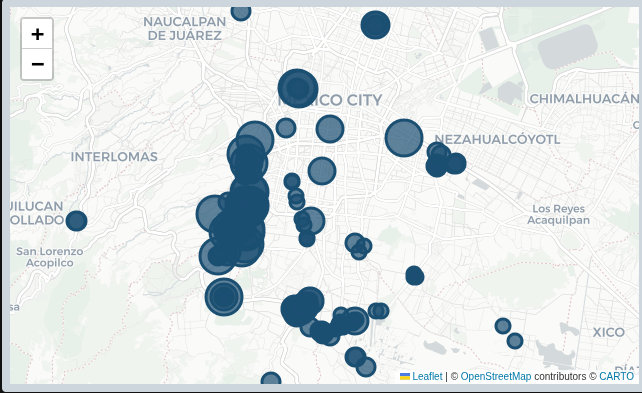
\includegraphics[width=0.8\textwidth, height=0.6\textheight, keepaspectratio]{../Ensayo_Humedales/img/FuerzaCapilarTotalNodosGoegraficosDispersos.png}
    \caption{Fuerza Capilar Total Mapeada a través de Nodos Geográficos \cite{garibaldi2023vft}.}
    \fuentefigura{Elaboración propia.}
  \end{figure}
\end{frame}

% ── Diapositiva 4: Complejidad Regional ───────────────────────────────────────
\begin{frame}{Contexto Regional y Administrativo}
  \begin{itemize}
    \item \textbf{Ubicación:} Oriente de la CDMX.
    \item \textbf{Alcaldías involucradas:} Tláhuac, Xochimilco e Iztacalco.
    \item \textbf{Conectividad Metropolitana:} Vínculo directo con Nezahualcóyotl, Chimalhuacán y Texcoco (Edomex).
  \end{itemize}
  \begin{figure}
    \centering
    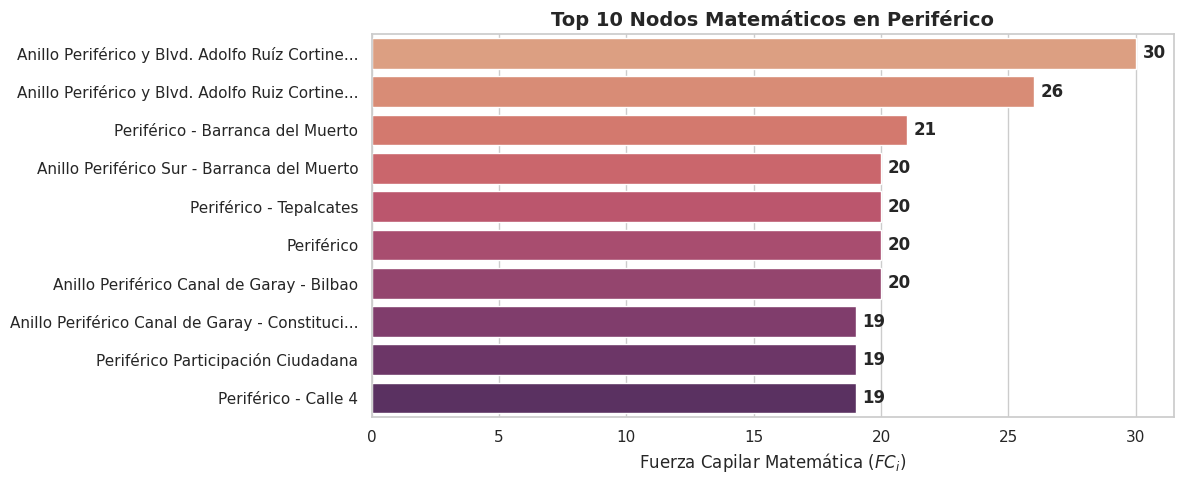
\includegraphics[width=0.7\textwidth, height=0.45\textheight, keepaspectratio]{../Ensayo_Humedales/img/MacroHubsFuerzaCapilarAnilloPerifericoGrafica.png}
    \caption{Macro-Hubs de Fuerza Capilar sobre el Anillo Periférico.}
  \end{figure}
\end{frame}

% ── Diapositiva 5: Teoría del Corredor Circular ───────────────────────────────
\begin{frame}{El Corredor Circular como Barrera Estructural}
  \begin{itemize}
    \item \textbf{Más que transporte:} Es una \textit{barrera artificial estructural}.
    \item \textbf{Optimización Matemática:} Consolidar la transferencia en puntos específicos evita la dispersión hacia zonas protegidas.
    \item \textbf{Protección del Patrimonio:} El límite físico refuerza legalmente las Áreas Naturales Protegidas (ANP).
    \item \textbf{Conclusión Teórica:} La movilidad masiva actúa como herramienta de defensa contra la urbanización fragmentada \cite{garibaldi2023vft}.
  \end{itemize}
\end{frame}

% ── Diapositiva 6: Mapa Final (Figura 3) ──────────────────────────────────────
\begin{frame}{Intersección Crítica: Periférico y Humedales}
  \begin{figure}
    \centering
    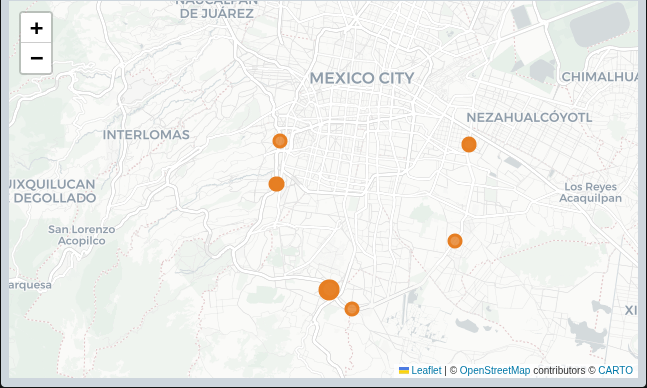
\includegraphics[width=0.8\textwidth, height=0.7\textheight, keepaspectratio]{../Ensayo_Humedales/img/MapaFuerzaCapilarAnilloPerfericoLimpio.png}
    \caption{Mapa de Fuerza Capilar: Nodos críticos en humedales urbanos.}
    \fuentefigura{Garibaldi (2023).}
  \end{figure}
\end{frame}